\chapter{Introducción}\label{cap1}

\section{Contexto} \label{sec:intro-contexto}
Todos los institutos de salud pública en México cuentan con proveedores que se encargan de surtir los medicamentos a sus respectivas clínicas y hospitales. El documento digital en el cual se asienta la solicitud de un medicamento es llamada \textit{orden de reposición}; este documento contiene la descripción del medicamento y el lugar en donde es solicitada la entrega del mismo. En particular, el \textit{Instituto} para el cual se realiza este proyecto hace llegar a los proveedores las órdenes de reposición a través de su sistema web llamado \textit{Sistema de Abastecimiento}. Dentro de éste, el proveedor, a su vez, puede confirmar la recepción de las órdenes de reposición.\\
El proveedor tiene operadores dedicados a interactuar con el \textit{Sistema de Abastecimiento}. Las tareas que debe cumplir el operador del \textit{Sistema de Abastecimiento} son: confirmar la recepción de órdenes de reposición al \textit{Sistema de Abastecimiento}, obtener la información necesaria para cumplir con la entrega del medicamento (Figura \ref{fig:flow-proc-contestar}) y extraer las órdenes de reposición que han sido canceladas (Figura \ref{fig:flow-proc-verificar}), lo cual significa que el \textit{Instituto} ya no requiere el medicamento especificado en la orden de reposición y, de ser entregadas, serán rechazadas.\\
El proveedor realiza dos tipos de procesos:
\begin{enumerate}
\item \textbf{Envío de órdenes de reposición}. Un operador accede al \textit{Sistema de Abastecimiento}, con un usuario y contraseña previamente asignados, posteriormente se dirige a la sección \textit{Contestación a Órdenes de Reposición}, que es donde se muestra un listado con las órdenes de reposición emitidas por el \textit{Instituto} que aún no han sido atendidas. El operador manualmente ingresa en cada orden de reposición los datos requeridos: la cantidad de unidades que enviará, fechas de fabricación y de caducidad. A esto se le conoce como responder la orden reposición.\\
Cuando una orden de reposición ha sido \textit{contestada}, en el listado de órdenes de reposición de la sección \textit{Contestación a Órdenes de Reposición} se muestra la opción de ``enviar''. Aquí el operador selecciona la opción ``enviar'' de cada una de las órdenes de reposición que ha contestado, el \textit{Sistema de Abastecimiento} muestra el formato de acuse de recibo, el operador extrae los datos de interés que se muestran en el acuse y hace una impresión de la pantalla. El flujo descrito anteriormente se muestra en la Figura \ref{fig:flow-proc-contestar}.

\begin{figure}[H]
\centering
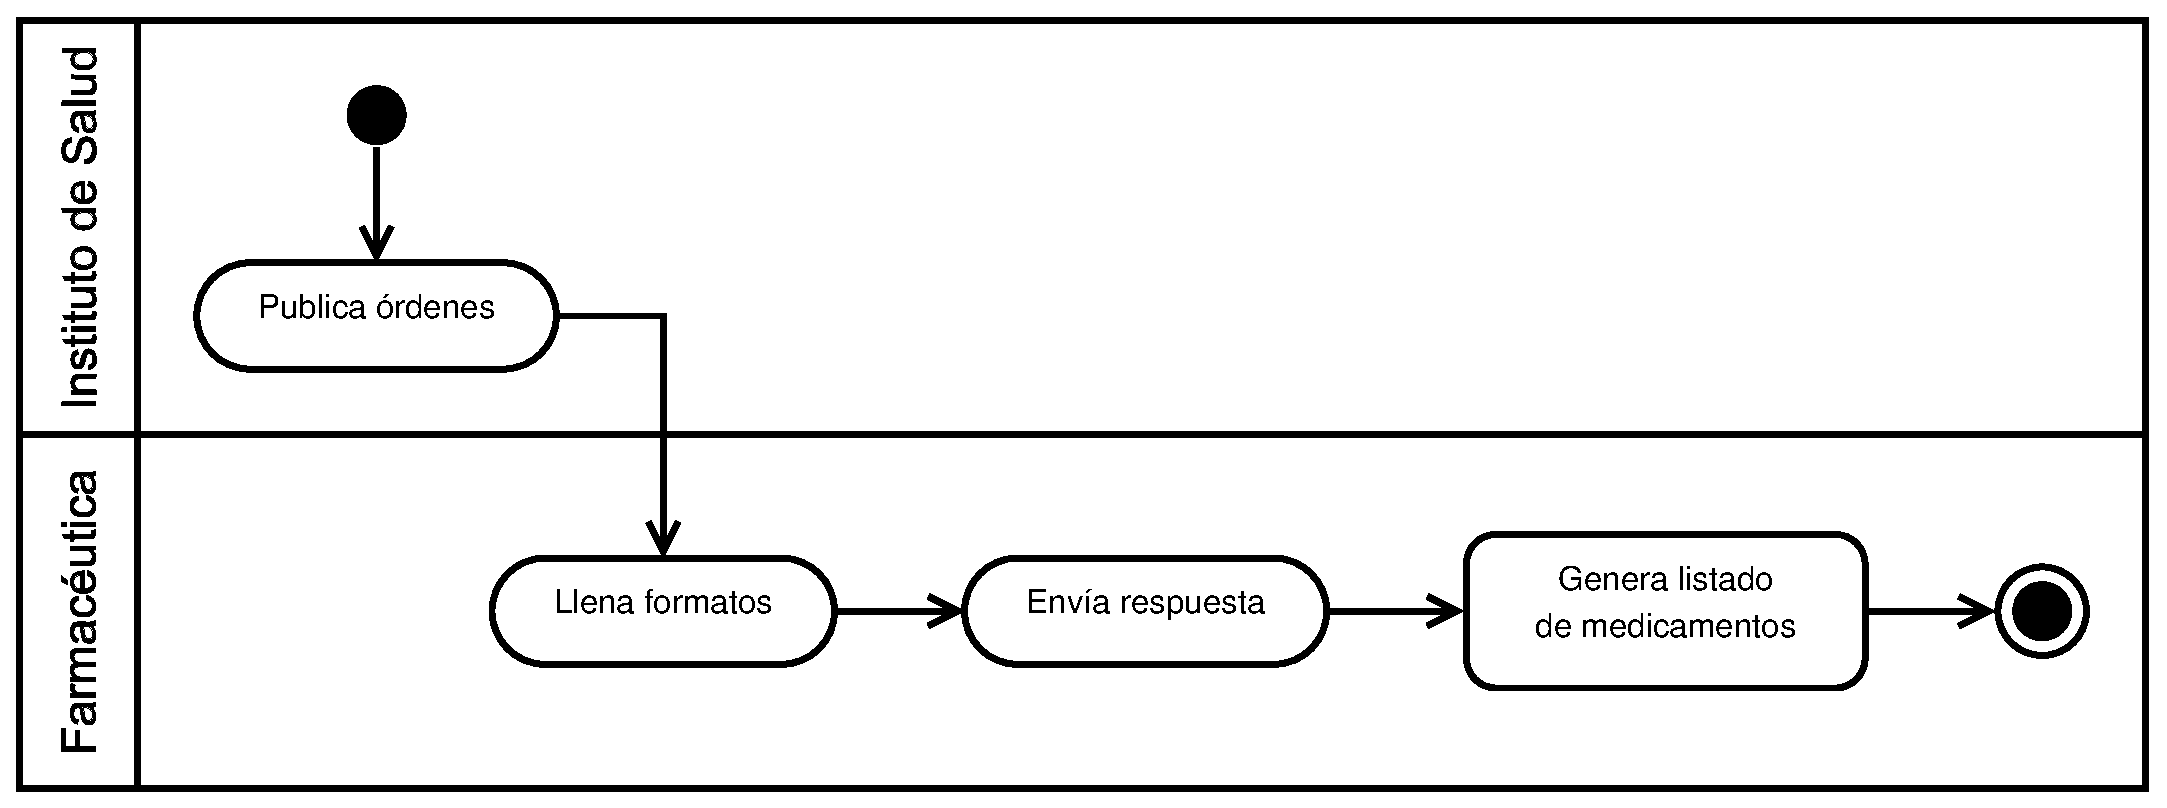
\includegraphics[scale=0.4]{flow-proc-contestar} 
\caption{Flujo del proceso para contestar órdenes de reposición.}
\label{fig:flow-proc-contestar}
\end{figure}

\item \textbf{Verificación de órdenes de reposición canceladas}. Dado que el \textit{Instituto} tiene la facultad de cancelar las órdenes aun cuando ya hayan sido enviadas, es importante para el proveedor evitar el gasto extra que implica retirar medicamento no solicitado que ya ha sido enviado al \textit{Instituto}. El operador accede al \textit{Sistema de Abastecimiento} de la misma manera como se describe en el punto anterior, se dirige a la sección \textit{Consulta de Órdenes}, donde provee información para realizar la búsqueda: rango de fechas de emisión\footnote{Fecha en que la orden fue realizada.}, el estado de la orden como ``cancelada''. Como resultado de esta búsqueda, se muestra un listado con las órdenes que cumplen con tal filtro. El operador copia la lista en un documento en su equipo personal, para posteriormente extraer las órdenes de reposición que han sido canceladas de las cuales no se tenía conocimiento. En la Figura \ref{fig:flow-proc-verificar} se muestra el proceso para verificar las órdenes de reposición canceladas.
\begin{figure}[H]
\centering
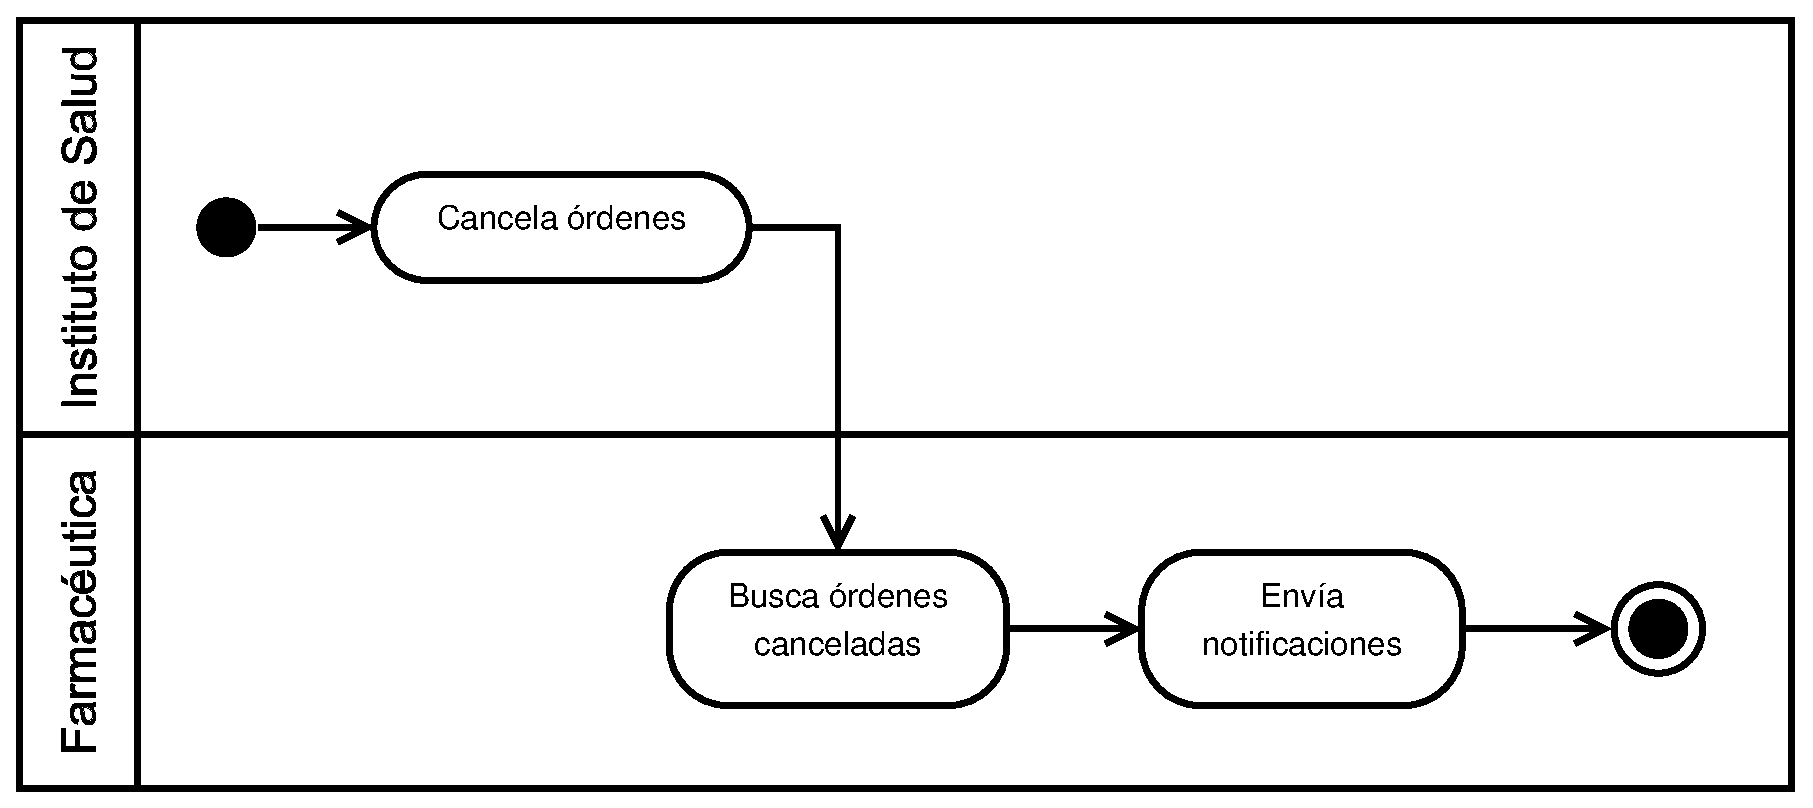
\includegraphics[scale=0.4]{flow-proc-verificar} 
\caption{Flujo del proceso para verificar órdenes de reposición canceladas.}
\label{fig:flow-proc-verificar}
\end{figure}
\end{enumerate}

En este documento se hará referencia de manera indistinta al proveedor\footnote{Quien requiere automatizar la interacción con el Sistema de Abastecimiento para el envío de las órdenes de reposición y la verificación de órdenes canceladas.} como la compañía farmacéutica o simplemente como farmacéutica.\\
Para completar las tareas de envío de órdenes de reposición y verificar las órdenes de reposición canceladas dentro del \textit{Sistema de Abastecimiento}, la farmacéutica dedica diariamente un equipo constituido por tres personas durante toda la jornada laboral. Dependiendo del volumen de órdenes de reposición emitidas por el \textit{Instituto} se puede agregar una persona más al equipo.

\section{Objetivos}
\subsection{Objetivo principal}\label{sec:objetivo-principal}
Describir un sistema de cómputo --de ahora en adelante llamado \textbf{AutoSA}-- que reduzca el tiempo de interacción entre los operadores de la farmacéutica y el \textit{Sistema de Abastecimiento}. Es así que el sistema AutoSA busca cumplir las siguientes metas:
\begin{enumerate}
	\item Reducir el tiempo utilizado para contestar las órdenes de reposición.
	\item Evitar el envío de medicamentos cuyas órdenes de reposición hayan sido canceladas.
	\item Agilizar la generación de reportes sobre las órdenes de reposición atendidas.
\end{enumerate}

\subsection{Objetivos secundarios}\label{sec:objetivos-secundarios}
\begin{enumerate}
\item Reducir el error humano en relación con la manipulación de la información.
\item Ahorrar recursos en la entrega de medicamentos no solicitados.
\item Reducir el tiempo de respuesta a las órdenes de reposición.
\item Dar consistencia en los datos respecto a la generación de reportes estadísticos sobre las órdenes de reposición procesadas.
\end{enumerate}
Por lo anterior, los afiliados del \textit{Instituto} se verán beneficiados pues los medicamentos estarán disponibles con mayor frecuencia en las clínicas y hospitales.

\section{Descripción general de trabajo}\label{sec:desc-general}
La farmacéutica atiende las órdenes de reposición del \textit{Instituto} en el doble de tiempo que su competencia, en particular contestar estas órdenes en el \textit{Sistema de Abastecimiento} requiere diariamente de tres personas dedicadas durante toda la jornada laboral para terminar esta parte del proceso. La solución propuesta para acelerar la respuesta y verificación de órdenes de reposición del \textit{Sistema de Abastecimiento} se encuentra programado por agentes\footnote{Agente dentro de este trabajo se refiere a las rutinas que automatizan los procesos realizados por los operadores del \textit{Sistema de Abastecimiento}.}. Cada agente se dedica a emular las acciones del operador de la farmacéutica, el cual es el responsable de contestar o verificar las órdenes de reposición. El sistema AutoSA cuenta con una base de datos donde se almacenan los datos capturados por los agentes durante la respuesta de órdenes y una interfaz gráfica donde los trabajadores de la farmacéutica puedan realizar tareas de administración. Estas tareas pueden ser: la búsqueda, la edición de órdenes de reposición y la generación de reportes de las órdenes atendidas por los agentes.\\
La automatización de los procesos (Figuras \ref{fig:flow-proc-contestar} y \ref{fig:flow-proc-verificar}) antes mencionados pronostica una reducción de costos por devolución de medicamento no solicitado para el cliente y también la disminución de pérdidas en las ventas por solicitudes no atendidas en los rangos de tiempo acordados con el comprador. Dado lo anterior, se plantea un proyecto de software que cubra las necesidades de automatización y pueda ser administrado por usuarios no especializados en computación.\\
Para resolver el desarrollo del proyecto, el sistema AutoSA se divide en módulos con funcionalidades específicas que se muestran a continuación:
\begin{enumerate}
\item \textbf{Automatización de interacción con el Sistema de Abastecimiento}. La automatización de la interacción con el \textit{Sistema de Abastecimiento} consiste en replicar los pasos que sigue el operador de la farmacéutica en el llenado y extracción de información de las órdenes de reposición del \textit{Sistema de Abastecimiento}, es decir, listar los pasos que sigue el operador cuando contesta las órdenes de reposición; describir las reglas de negocio necesarios para llenar los formularios que presenta el \textit{Sistema de Abastecimiento} al responder una orden de reposición; por último, se identifican las fuentes de los datos que se ocupan para llenar tales formularios y se define la forma de almacenamiento de la información necesaria de cada formulario.
\item \textbf{Generación de reportes}. La generación de reportes consiste en plasmar la información obtenida de las órdenes de reposición contestadas en el módulo anterior. La farmacéutica tiene ya una plantilla que se utiliza para pasar los pedidos a otras áreas, con el fin de continuar la atención de las órdenes de reposición; además de obtener estadísticas relacionadas con la cantidad de órdenes de reposición atendidas y canceladas.
\item \textbf{Interfaz de usuario}. La interfaz de usuario se refiere a la aplicación que muestra una interfaz gráfica en la cual los operadores de la farmacéutica pueden solicitar la generación de reportes, hacer consultas y modificaciones a las órdenes de reposición atendidas por el primer módulo.
\end{enumerate}

\subsection{Arquitectura de la solución}
Una definición de arquitectura de software es dada por Bourque\cite{SWEBOOK}:
\begin{quote}
El conjunto de estructuras necesarias para la comprensión de un sistema en el cual se comprometen elementos de software, relaciones entre ellos y sus propiedades.
\end{quote}
Esta definición expone que los requerimientos del cliente se traducen en especificaciones técnicas para los desarrolladores. Aplicando la definición anterior al presente proyecto donde tenemos los siguientes componentes (Figura \ref{fig:dia-package-small}):
\begin{figure}[h]
\centering
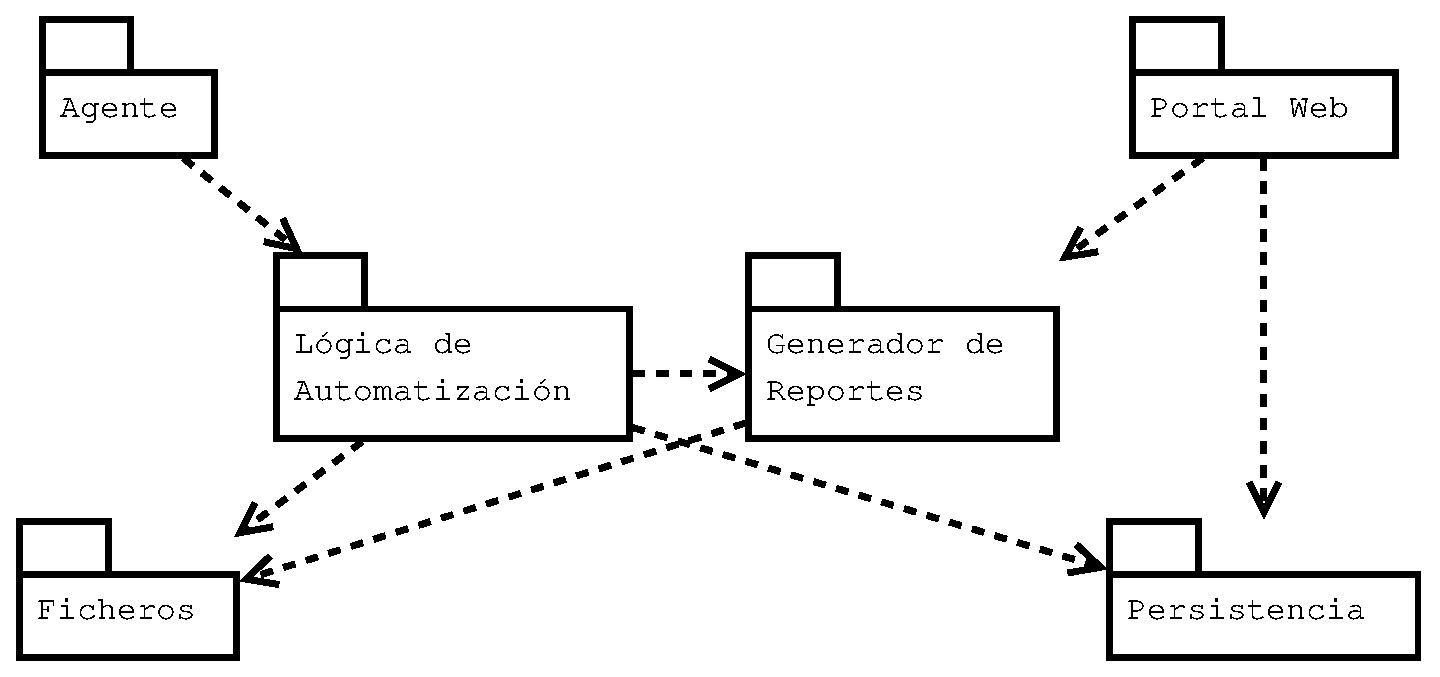
\includegraphics[scale=0.5]{dia-package-small} 
\caption{Módulos de la arquitectura.}
\label{fig:dia-package-small}
\end{figure}
\begin{itemize}
\item \textbf{Agente (robot)}. Interactúa directamente con el \textit{Sistema de Abastecimiento}, es el componente que automatiza las acciones de los operadores humanos de la farmacéutica.
\item \textbf{Lógica de Automatización}. Son bibliotecas y rutinas que se encargan de prestar los servicios necesarios al agente para su funcionamiento. Permite comunicación con la base de datos, guarda las capturas de pantalla en el sistema de archivos y provee la configuración de inicio al agente.
\item \textbf{Persistencia}. Es el componente que se encarga de llevar la persistencia de los datos obtenidos durante la respuesta a las órdenes de reposición.
\item \textbf{Ficheros}. Este componente es el encargado de manejar operaciones con el sistema de archivos para almacenar las capturas de pantalla al momento de enviar la respuesta de cada orden de reposición.
\item \textbf{Generador de Reportes}. Este módulo está encargado de la generación de reportes, tales como: órdenes de reposición atendidas, canceladas y formatos de órdenes de reposición enviadas.
\item \textbf{Portal Web}. Portal mediante el cual los usuarios pueden hacer correcciones a los datos obtenidos de las órdenes de reposición, reimprimir el formato de envío de la orden de reposición  y descargar los reportes generados por el módulo generador de reportes.
\end{itemize}
\subsection{Metodología utilizada}
El proyecto es abordado con la metodología \textit{Scrum}, la cual es un marco de trabajo para desarrollar, entregar y mantener productos complejos. Ésta consiste en un conjunto de roles, eventos, artefactos y reglas que los ligan. \textit{Scrum} da un enfoque adaptivo mientras promueve la entrega continua de soluciones y divide el desarrollo en ventanas de tiempo llamadas \textit{sprint}\cite{scrum}.\\
Dentro de \textit{Scrum} destacan los siguientes roles utilizados para el desarrollo del proyecto AutoSA\cite{scrum}:
\begin{itemize}
	\item \textit{Product Owner}: es responsable de maximizar el valor del producto que resulta del trabajo del \textit{Development Team}. Es la persona encargada de mantener el conjunto de tareas pendientes para futuros \textit{sprints}.
	\item \textit{Development Team}: es un grupo de profesionales encargado de realizar el trabajo necesario para completar las entregas de cada \textit{sprint}.
	\item \textit{Scrum Master}: es la persona responsable de promover y soportar \textit{Scrum} como está definido en la guía de \textit{Scrum}. Es un líder servil para el \textit{Scrum Team} que auxilia a este último a maximizar el valor del producto creado y ayuda a los involucrados en el desarrollo a comprender \textit{Scrum}.
	\item \textit{Scrum Team}: es conformado por el \textit{Product Owner}, el \textit{Development Team} y el \textit{Scrum Master}. \textit{Scrum Team} es un equipo de trabajo autoorganizado y multifuncional. Está diseñado para optimizar la flexibilidad, creatividad y productividad sin depender de personas ajenas al equipo.
	\item \textit{Stakeholder}: esta definición proviene directamente de su significado en inglés, refiere a las personas que tienen interés en el producto.
\end{itemize}
El grupo de trabajo (\textit{Scrum Team}) formado por la consultora para el proyecto AutoSA consta de dos personas:
\begin{enumerate}
	\item Desarrollador: es la persona que cumple con las funciones siguientes:
	\begin{enumerate}
		\item Levantar los requerimientos de los \textit{stakeholders} de la farmacéutica.
		\item Cumplir con el rol de \textit{Product Owner} al ser encargado de mantener la lista de tareas para los \textit{sprints} futuros.
		\item Hacer investigación sobre tecnologías adecuadas para el desarrollo.
		\item Realizar el diseño e implementación de los componentes del sistema AutoSA.
		\item Formar parte del \textit{Scrum Team}.
	\end{enumerate}
	\item Arquitecto: tiene las siguientes responsabilidades:
	\begin{enumerate}
		\item Supervisar y aprobar el diseño e implementación realizado por el desarrollador.
		\item Hacer investigación sobre tecnologías adecuadas para el desarrollo.
		\item Cumplir con el rol de \textit{Scrum Master}.
		\item Formar parte del \textit{Scrum Team}.
	\end{enumerate}
\end{enumerate}
El proyecto fue planeado para ser realizado de julio a diciembre de 2014. Su conclusión es la liberación del sistema AutoSA que consiste en el despliegue total de los módulos en el ambiente productivo provisto por la farmacéutica dando como resultado los siguientes productos:
\begin{itemize}
\item Rutinas para la generación de objetos en base de datos.
\item Rutinas para la creación de la estructura de directorios en el sistema de archivos.
\item Archivos de configuración propios de cada módulo.
\item Herramienta y rutinas de automatización.
\item Bibliotecas del portal web.
\item Manual de instalación y de usuario.
\item Capacitación a usuarios finales.
\end{itemize}
El autor del presente documento cumplió con rol de desarrollador desde el inicio del proyecto AutoSA hasta su liberación.\\
En síntesis, el \textit{Instituto de Salud}, mediante su \textit{Sistema de Abastecimiento}, realiza las órdenes de reposición de medicamentos a las farmacéuticas. Estas últimas invierten veinticuatro horas hombre por día para lograr contestar todas las órdenes de reposición. Reducir el tiempo en que se contestan las órdenes de reposición aumenta la velocidad de respuesta de la farmacéutica para entregar los medicamentos a centros de salud del \textit{Instituto}, motivo por el cual le interesa automatizar esta parte. El sistema AutoSA que se propone en este documento da solución mediante dos subsistemas: uno que automatiza los procedimientos de interacción con el \textit{Sistema de Abastecimiento} y otro que permite al personal de la farmacéutica generar reportes y acceder a datos de las órdenes de reposición atendidas.